\documentclass[11pt,a4paper]{article}
\usepackage{float}
\usepackage{verbatim}
\usepackage{subfig}
\usepackage[T1]{fontenc}
\usepackage[utf8]{inputenc}
\usepackage{geometry}
\usepackage{enumitem}
\geometry{verbose,lmargin=2cm,rmargin=2cm, bmargin=2cm, tmargin=2cm}
\usepackage{wrapfig}
\usepackage{tikz}
\usetikzlibrary{decorations.markings}
\usepackage{calc}
\usepackage{wrapfig}
\usepackage{graphicx}
\usepackage{amssymb}
\usepackage{amsmath}
\usepackage{esint}
\usepackage{hyperref}
\begin{document}

%\preprint{APS/123-QED}

\title{Lab Report: Length, Velocity and Acceleration}% Force line breaks with \\

\author{Nicholas Karlsen}
% \email{nichoka@student.matnat.uio.no}

\date{\today}% It is always \today, today,
             %  but any date may be explicitly specified

\maketitle

%\tableofcontents
\begin{abstract}
  A study on different methods for determining the length, velocity and acceleration of different objects, and the errors involved in these methods.
\end{abstract}
\section{\label{sec:intro}Introduction}

\section{\label{sec:theory}Theory}
  \subsection{Pendulum}
    \begin{equation}
      \label{eqn:period}
        T \approx 2\pi \sqrt{\frac{L}{g}}\enspace
    \end{equation}
    Where $T$ denotes the period of a pendulum, $L$ its length and $g$ the gravitational acceleration. The small angle approximation (Eqn. \ref{eqn:period})  is valid for angles $\theta \ll 1\, \textup{rad}$ with an error $\approx \pm 15 \, \textup{s}$ per day \cite{pend_wik}.

  \subsection{Doppler shift}
    \begin{equation}
      f_m = f + \Delta f = \frac{c}{c-v}f  
    \end{equation}
    Where $f_m$ denotes a measured frequency from an observer at rest, $f$ the frequency in the rest frame of a body moving relative to an observer, $\Delta f$ the doppler shift, $c$ the speed of sound in air and $v$ the velocity of the body relative to the observer.

  \subsection{Errors}
    \begin{equation}
    \label{eqn:sigma}
      \sigma \approx \left(
      \frac{\sum x_i^2 - \frac{1}{n}(\sum x_i)^2}
      {n - 1}
      \right)^\frac{1}{2}
    \end{equation}
    
    \begin{equation}
      \label{eqn:sigma_m}
      \sigma_m \approx \left(
      \frac{\sum x_i^2 - \frac{1}{n}(\sum x_i)^2}
      {n(n - 1)}
      \right)^\frac{1}{2}
    \end{equation}

    Where $\sigma, \sigma_m$ denotes the standard deviation, and the standard deviation of the mean respectively of a set of $n$ values $x_i$. \cite{squires}.

    Any errors stated in a derived number will be calculated using the equations for combinations of errors found on page 29 in Squires \cite{squires}. Lastly, when using a linear fit on a set of linearly correlated data i used the expressions found on page 39 in Squires \cite{squires} to calculate the regression line, as well as its error.

\section{\label{sec:exp_proced}Experimental Procedure}
 
  \subsection{Measuring the difference in lengths between two rods}
    \subsubsection{Measurements using the Hultafors meter ruler}
      The rod was placed on a flat surface, and the end of the rod was lined up with the $1cm$ marker on the Hultafors Meter ruler in order to negate any effect the "wear and tear" of the ruler might have on the results. This $1cm$ difference was accounted for in our reading of the data. The ruler was laid down on the table along with the rod, and did flex slightly because of this. The error due to flex is accounted for in the error section of the data sheet provided by the manufacturer. This procedure was repeated for both rods a and b.

    \subsubsection{Measurements using the Bosch PLR30}
      The rods were placed and secured to the table using adhesive tape on a table whilst being in direct contact with a wall. The Bosch PLR30 Laser rangefinder \cite{PLR}, henceforth referred to as "laser", was then placed at the opposing end of the rod in order to measure the length from there, to the wall. Since the rod was touching the wall, this effectively means that we measured the length of the rod. There was a slight degree of systematic error in our procedure, as we could not ensure that the laser was pointing with exact parallel to the rod, nor did we have an exact way of placing the laser such that its origin would be at the exact end-point of the rod. 

    \subsection{Measurement using a digital vernier caliper}
      In order to determine the difference in length between the two rods directly we used a digital vernier caliper \cite{cocraft}. The rods were secured to a table in parallel, right next to each other with the ends on one side lined up with each other. The measurement of the difference in their lengths was then made on the other side using the vernier caliper. The vernier caliper was held above the two rods, resting on them in order to minimize any systematic error.

  \subsection{Measuring the period and height of the Foucault's pendulum}

    \subsubsection{\label{subsect:exp_period}Measuring the period of the pendulum}
    The measurements were taken in sequence using the lap function of the Cielo 100MT \cite{cielo} stopwatch. The time was recorded every other apex of the swing, which amounts to one period. All of the measurements were taken by the same person in order to ensure that the error in judgment and reaction time would remain the same throughout all of the measurements.

    \subsubsection{Measuring the height of the center of mass}
      In order to perform this measurement two people stood on opposing sides of the enclosure, as shown in Fig \ref{fig:pendelfy}. One rested a meter ruler up against the glass enclosure and standing on the floor, whilst the other pointed a laser from the other side. The laser was pointed to the meter ruler whilst held hotizontaly. Then, while the pendulum was still in motion, the laser was progressively adjusted during each swing untill it was just below the lowest point of the pendulums trajectory, reapeated this to fi. Needless to say, this is a highly inaccurate measurement, and there is no percise way to determine the magnitude of the error in this reading as it is almost entirely due to a systematic fault in our method.
      \begin{figure}[H]
        \center 
        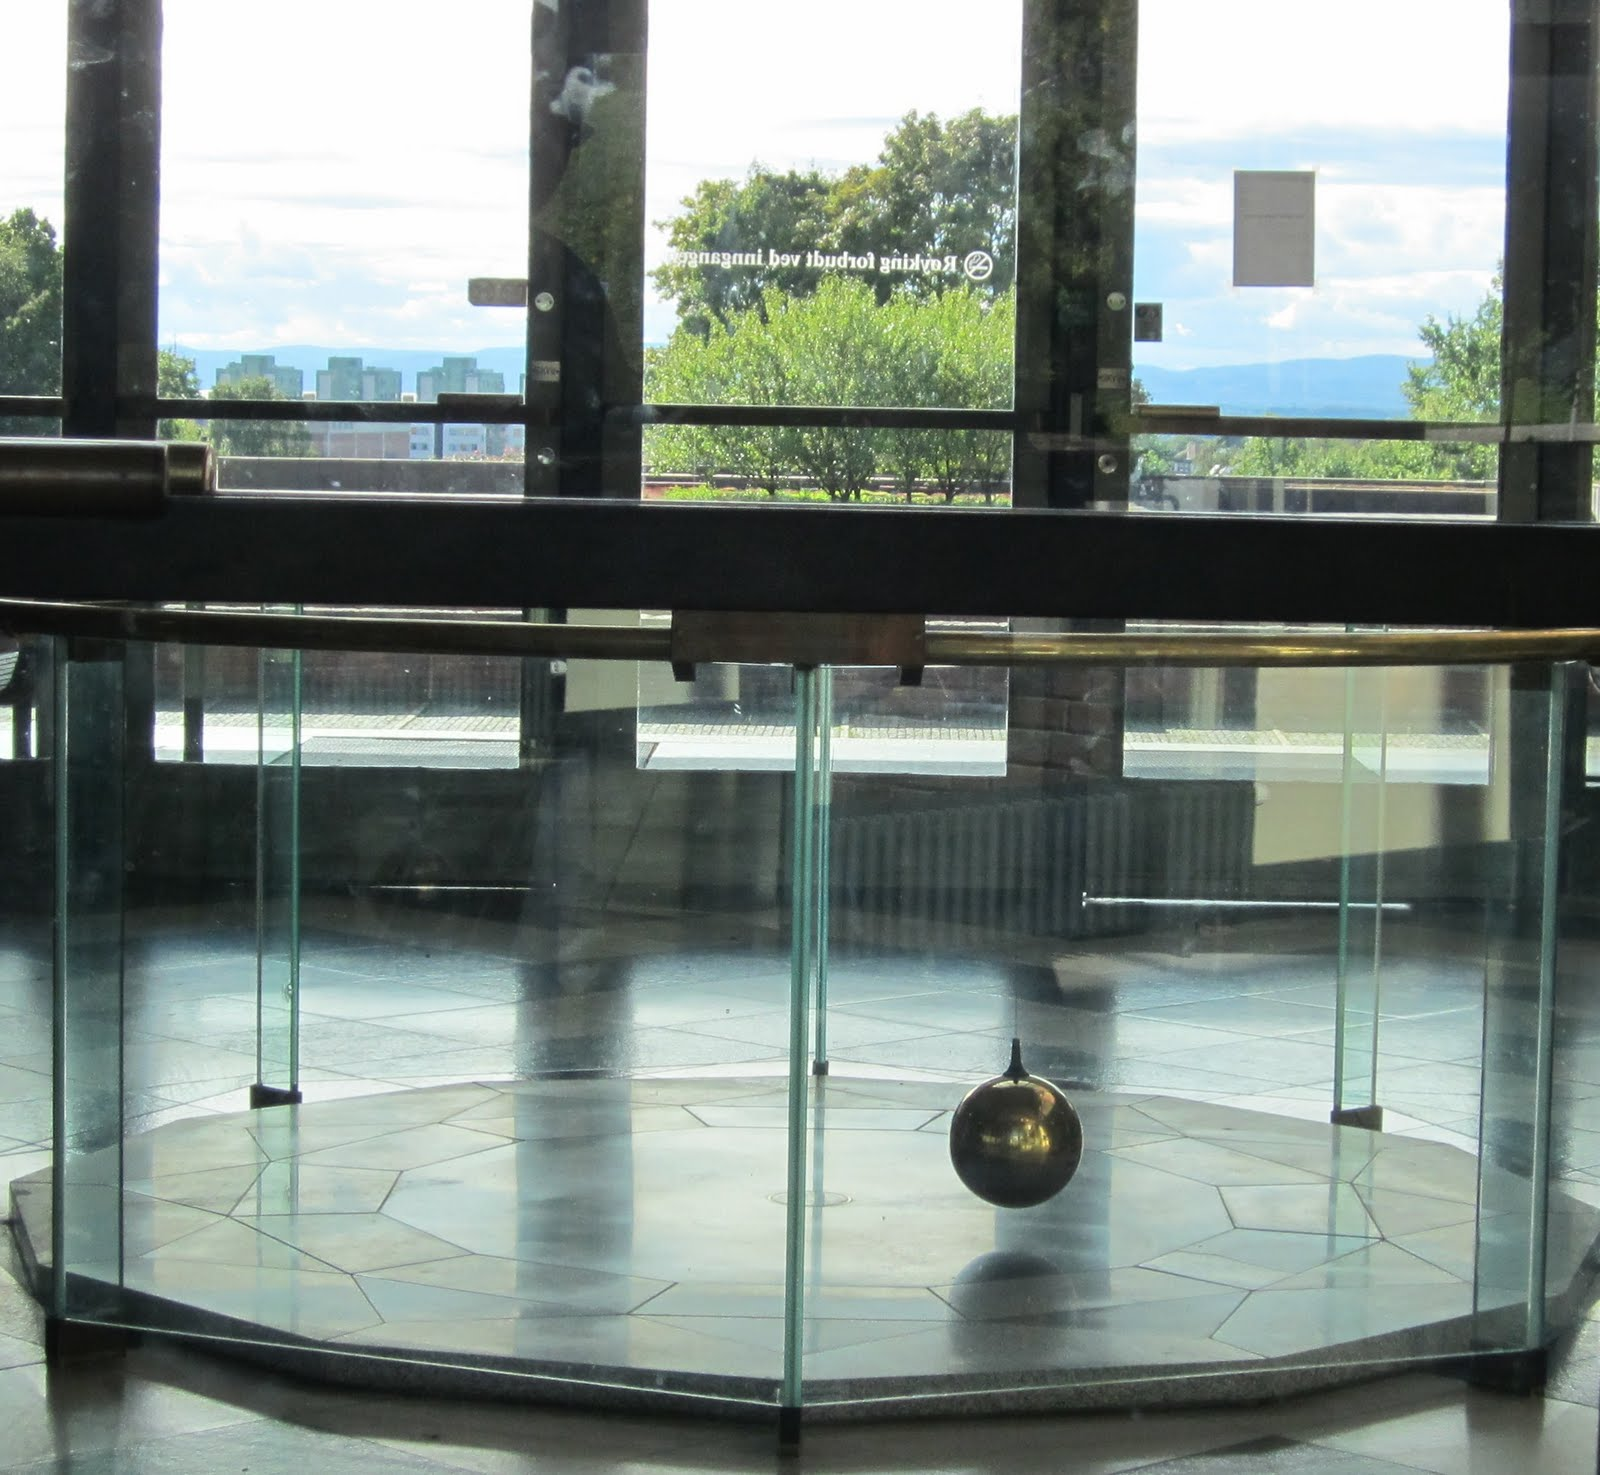
\includegraphics[scale=0.15]{scripts/figs/pendelimg.JPG}
        \caption{A photograph of the Focault's Pendulum at UiO.}
        \label{fig:pendelfy}
      \end{figure}

    \subsubsection{Measuring the height of the roof}
      The Laser rangefinder \cite{PLR} was placed on the floor of the entrance hall, turned on and the measured value was recorded in the lab journal.


  \subsection{Measuring the acceleration of a lego-car}
    A model car made of lego, with an attatched speaker emitting a sound with constant frequency was placed on a ramp with variable height and constant length as sketched in Fig. \ref{fig:rampsketch}.
    \begin{figure}[H]
      \center
      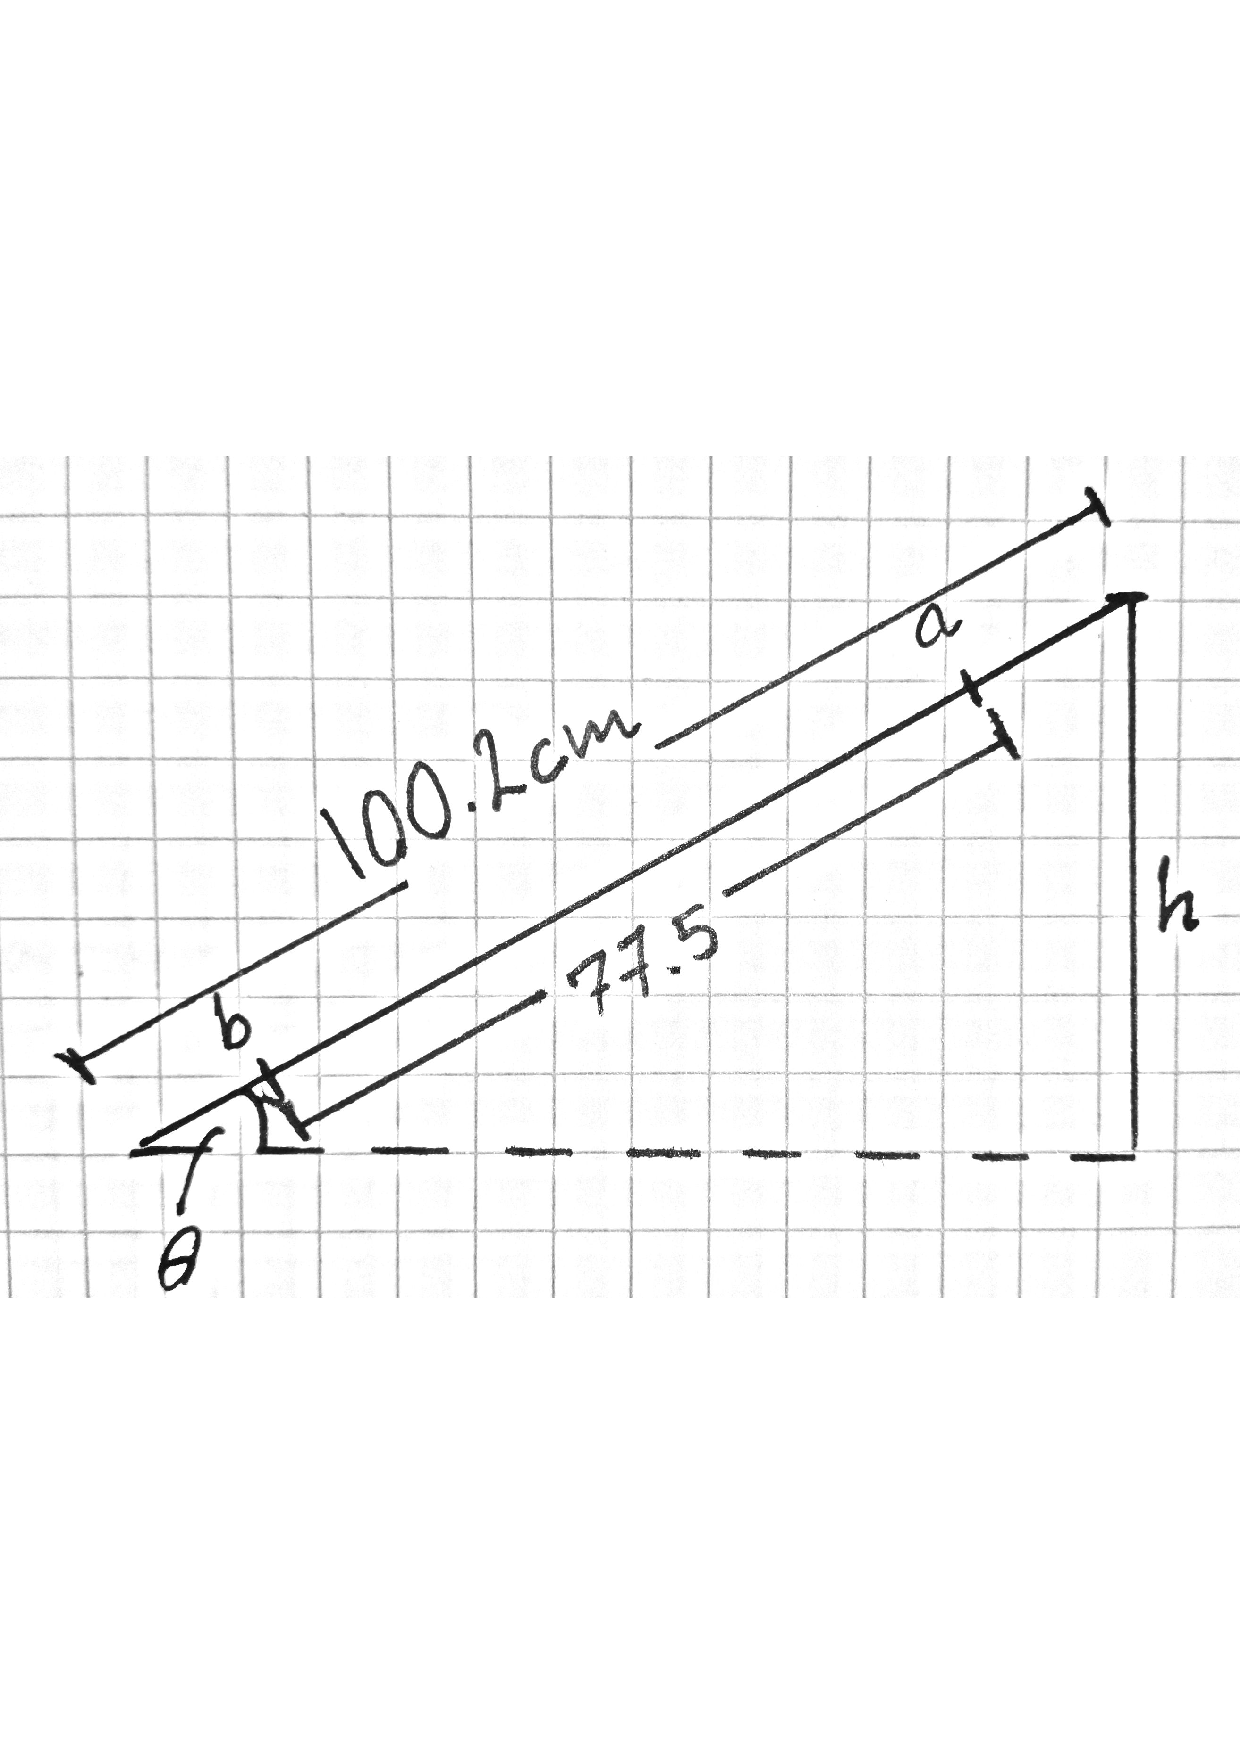
\includegraphics[scale=0.3]{scripts/figs/legodiag.pdf}
      \caption{Sketch showing the properties of the ramp used}
      \label{fig:rampsketch}
    \end{figure}
    The model car was released with its nose at point a (marked with black adhesive tape) and accelerated by gravity until its nose hit point b (also marked with black adhesive tape). This was timed using a stopwatch by the same person who made the measurements in section \ref{subsect:exp_period}. At the bottom of the ramp there was a microphone connected to a PC with matlab which collected sound data. Several people conducted similar experiments in the same room and at the same time, so the microphone may have picked up other signals as well.

    The experiment was repeated 3 times, with varying heights, $h$.
  
  \subsection{Measuring the velocity of the RC-car}
    An RC-Car with an attached speaker emitting a sound with constant frequency was driven along the floor. The sound was recorded with a microphone connected to a PC running matlab. The car was driven on a linoleum floor, so its wheels did not grip as well as one might hope. It was also not driven perfectly straight, so the maximum velocity of the car may not have been reached. There was also not much room for the car to reach this velocity either.


\section{\label{sec:data} Results}

  \subsection{Rod measurements}
  \begin{table}[H]
    \center
    \caption{Length of rods}
    \label{tab:lenrods}
    \begin{tabular}{rrrrrrrrr}
\hline
Ruler & Ruler & Ruler & Ruler & Laser & Laser & Laser & Laser & Vernier Calliper \\
   $l_a [cm]$ &  $\delta l_a$ [cm] &   $l_b$ [cm] &   $\delta l_b$ [cm] &   $l_a$ [cm] &   $\delta l_a$ [cm] & $l_b$ [cm] &   $\delta l_b$ [cm] & $l_{a, b}$ [mm] \\
\hline
           119.50 &              0.23 &           119.60 &              0.23 &           120.50 &              0.20 &           120.60 &              0.20 &                         1.25 $\pm 0.05$ \\
           119.50 &              - &           119.70 &              - &           119.60 &              0.20 &           119.80 &              0.20 &                         - \\
           119.45 &              0.37 &           119.60 &              0.37 &           119.50 &              0.20 &           119.70 &              0.20 &                         1.40 $\pm 0.05$\\
           119.40 &              - &           119.50 &              - &           119.40 &              0.20 &           119.60 &              0.20 &                         - \\
           119.43 &              0.40 &           119.55 &              0.40 &           119.40 &              0.20 &           119.60 &              0.20 &                         1.20 $\pm $0.6\\
           119.40 &              0.20 &           119.60 &              0.20 &           119.68 &              0.20 &           119.72 &              0.20 &                         1.80 $\pm $0.05\\
           119.40 &              0.27 &           119.50 &              0.27 &           119.90 &              0.20 &           119.70 &              0.20 &                         0.00 $\pm 0.05$\\
           119.45 &              0.35 &           119.65 &              0.35 &           130.60 &              0.20 &           130.20 &              0.20 &                         1.80 $\pm $0.05\\
           119.40 &              - &           119.60 &              - &           119.40 &              0.22 &           119.50 &              0.22 &                         - \\
           119.43 &              0.31 &           119.55 &              0.31 &             - &              - &             - &              - &                         1.50 $\pm 0.05$\\
\hline
\end{tabular}

  \end{table}
  Table. \ref{tab:lenrods} contains all the measurements made of the rods by the Tuesday group, copied from the \href{https://uio.instructure.com/courses/910/modules/items/13592}{image} posted on canvas. Some of the data was not clearly readable, and has therefore been omitted from this table. The measurements made by me and my lab parter are located in row 1.

  Using this data i calculated the following values.
  \begin{align}
    \begin{split}
      \textup{Ruler:} \\
      \bar{l_{a}} &= 119.43 \pm  0.01\,cm \\
      \bar{l_{b}} &= 119.58 \pm 0.02 \,cm \\
      \bar{l_{ab}}&= 0.14 \pm 0.014
    \end{split}
  \end{align}

  \begin{table}[H]
    \center
    \caption{Derived data}
    \begin{tabular}{| l | l | l | l | l | l | l | l | l | l |}
\hline
    -  & $\bar{l_{a}}$ & $\sigma_a$ & $\sigma_{m, a}$ & $\bar{l_{b}}$ & $\sigma_b$ & $\sigma_{m, b}$ & $\bar{l_{ab}}$ & $\sigma_{ab}$ & $\sigma_{m, ab}$ \\ \hline

    Ruler  & $\bar{l_{a}}$ & $\sigma_a$ & $\sigma_{m, a}$ & $\bar{l_{b}}$ & $\sigma_b$ & $\sigma_{m, b}$ & $\bar{l_{ab}}$ & $\sigma_{ab}$ & $\sigma_{m, ab}$ \\ \hline

    Laser  & $\bar{l_{a}}$ & $\sigma_a$ & $\sigma_{m, a}$ & $\bar{l_{b}}$ & $\sigma_b$ & $\sigma_{m, b}$ & $\bar{l_{ab}}$ & $\sigma_{ab}$ & $\sigma_{m, ab}$ \\ \hline

\end{tabular}
  \end{table}

  \begin{table}[H]
    \center
    \caption{Uncertainty in Length measurement using the meter ruler}
    \label{tab:uncert}
    \begin{tabular}{| l | l | l |}
\hline
 & $x$ & $\delta x$ \\
\hline
$l_a$                 & $119.5cm$ &    \\             
$l_b$                 & $119.6cm$ &    \\        
$dl_s$                &     & $1.4mm$   \\             
$\sqrt{n}\cdot dl_l$  &     & $0.5\sqrt{5}mm$   \\                  
$dl_m$                &     & $1.4mm$   \\                  
$\alpha l_a (T-25C)$  & $-0.156cm$ & $\sim 10^{-6}$   \\ 
\hline                

\end{tabular}

\begin{tabular}{| l | l | l |}
\hline
& $\sum x_i$ & $\sqrt {\sum \sigma x_i^2 }$ \\
\hline
$\sum l_a$ & 119.48cm & 2.27 \\
$\sum l_b$ & 119.58cm & 2.27 \\
\hline   
\end{tabular}
  \end{table}
  
  \begin{itemize}
    \item $l_a, \enspace l_b:$ Recorded length of rod $a$ and $b$ respectively
    \item $dl_s:$ Error due to aiming of the ruler
    \item $\sqrt n \cdot dl_l:$ Error due to curvature of joints
    \item $dl_m:$ Error due to precision of measuring lines
    \item $\alpha :\enspace 4\cdot10^{-5\circ} C^{-1}$, Coefficient of linear thermal expansion for glass fiber
  \end{itemize}

  \subsubsection{Pendulum measurements}
  \begin{table}[H]
    \center
    \caption{Period of pendulum}
    \label{tab:pendel}
    \begin{tabular}{rrrr}
\hline
   T [s]\\
\hline
    7.30\\ 7.72\\ 7.57\\ 7.43\\ 7.73\\ 7.27\\ 7.68\\ 7.60\\ 7.34\\ 7.75\\
    7.06\\ 7.32\\ 7.55\\ 7.29\\ 7.08\\ 7.82\\ 7.78\\ 7.44\\ 7.68\\ 7.46\\
\hline
\end{tabular}

  \end{table}
  \begin{figure}[H]
    \center
    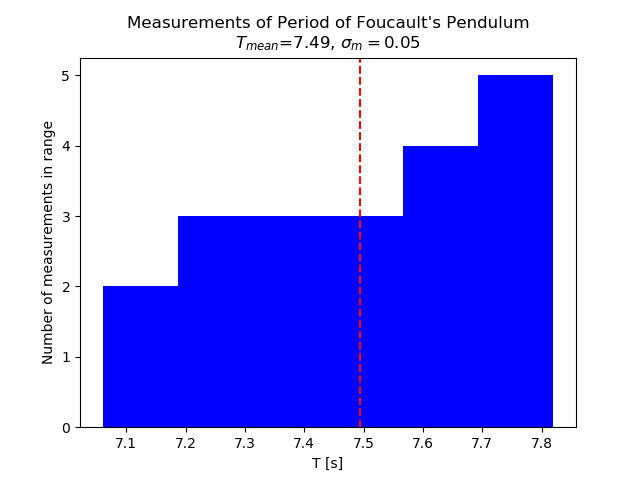
\includegraphics[scale=0.7]{scripts/figs/period.png}
    \caption{Measurements of the Period of the Foucault's Pendulum in the entrance hall at the Institute of Physics, UiO.}
    \label{fig:pendel}
  \end{figure}

  \subsubsection{Lego-car measurements}
    \begin{figure}[H]%
      \centering
      \subfloat[]{{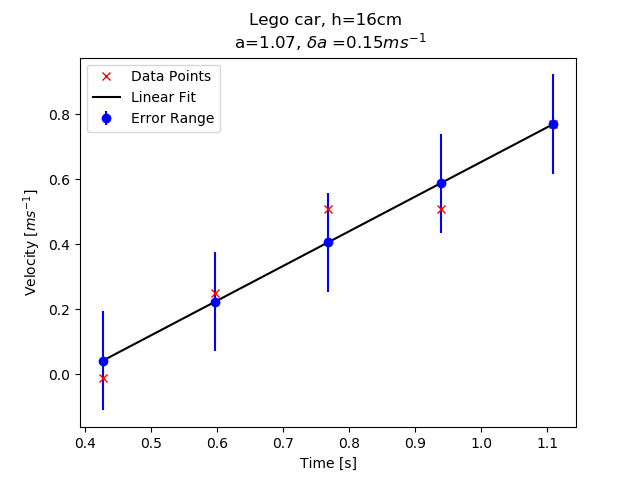
\includegraphics[width=9cm]{scripts/figs/lego16cm.png}}}
      \subfloat[]{{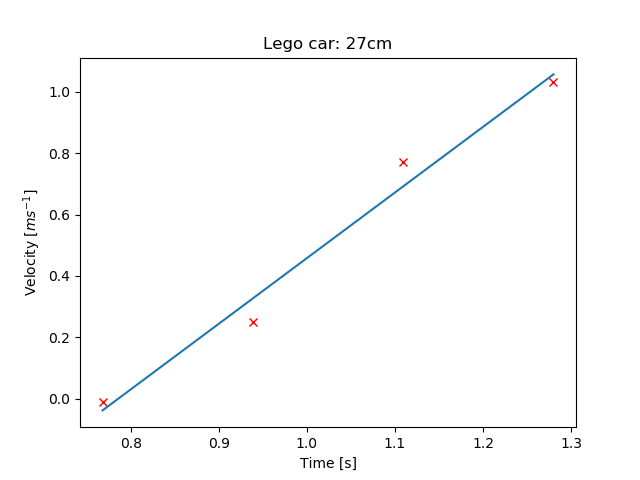
\includegraphics[width=9cm]{scripts/figs/lego27cm.png}}}
      \caption{}%
      \label{fig:vel_fit}%
    \end{figure}

  \subsubsection{RC-car measurements}


\section{\label{sec:disc}Discussion}
\section{\label{sec:conc}Conclusion}


\begin{thebibliography}{1}

\bibitem{pend_wik}
\url{https://en.wikipedia.org/wiki/Pendulum}.

\bibitem{squires}
G.~L. Squires.
\newblock {\em Practical Physics 4th Edition}.
\newblock Cambridge University Press, 2001.

\bibitem{cocraft}
\url{http://www.uio.no/studier/emner/matnat/fys/FYS2150/v18/kursmateriell/datablader-og-brukermanualer/cocraft-digitalskyvel%C3%A6r.pdf}

\bibitem{hultafors}
\url{http://www.uio.no/studier/emner/matnat/fys/FYS2150/v18/kursmateriell/datablader-og-brukermanualer/hultafors_meterstokk.pdf}

\bibitem{PLR}
\url{http://www.uio.no/studier/emner/matnat/fys/FYS2150/v18/kursmateriell/datablader-og-brukermanualer/bosch_plr30.pdf}

\bibitem{cielo}
\url{http://www.uio.no/studier/emner/matnat/fys/FYS2150/v18/kursmateriell/datablader-og-brukermanualer/stoppeklokke.pdf}

\end{thebibliography}

\end{document}